\documentclass[aspectratio=169,12pt]{beamer}
\usepackage{pgfpages}
\mode<presentation> {
  \usetheme{metropolis}
}

\usepackage{lipsum}
% \usepackage[colorgrid,gridunit=pt,texcoord]{eso-pic}
\usepackage[absolute,overlay]{textpos}
\usepackage{pythonhighlight}
\usepackage[absolute,overlay]{textpos}
\usepackage{url}
\usepackage{caption}
\usepackage{hyperref}
\usepackage[
    type={CC},
    modifier={by},
    version={3.0},
]{doclicense}
\usepackage[whole]{bxcjkjatype}
\usepackage{todonotes}
\usepackage{multimedia}

\setbeamertemplate{note page}{\pagecolor{yellow!5}\vfill\insertnote\vfill}
\setbeameroption{show notes on second screen=right}

\lstset{
language = Python,
breaklines = true,
basicstyle=\fontsize{7}{7}\selectfont\ttfamily,
commentstyle = {\itshape \color[cmyk]{1,0.4,1,0}},
keywordstyle = {\bfseries \color[cmyk]{0,1,0,0}},
stringstyle = {\ttfamily \color[rgb]{1,0,0}},
frame = single,
}
\hypersetup{
colorlinks=true,
}

\title{PyVista Contribution 2021}

\begin{document}
\author{Tetsuo Koyama}
\institute{PyVista developer team}

\frame{\titlepage}
\note{
こんにちは、Tetsuo Koyamaです。本日は、「PyVista Contribution 2021」というタイトルでお話します。
}

\begin{frame}[fragile]
\begin{textblock*}{350pt}(50pt, 20pt)
\begin{block}{Who am I?}
\note{
まずは自己紹介をさせてください。
}
\end{block}
\end{textblock*}
\begin{textblock*}{350pt}(50pt, 70pt)

\includegraphics[width=0.25\linewidth]{tkoyama010.png}
\end{textblock*}
\begin{textblock*}{350pt}(50pt, 170pt)

\includegraphics[width=0.05\linewidth]{twitter-5662063_1280.png}
\end{textblock*}
\begin{textblock*}{350pt}(70pt, 175pt)
\href{https://twitter.com/tkoyama010}{@tkoyama010}
\end{textblock*}
\begin{textblock*}{350pt}(50pt, 200pt)
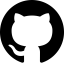
\includegraphics[width=0.05\linewidth]{github.png}
\end{textblock*}
\begin{textblock*}{350pt}(70pt, 205pt)
\href{https://github.com/tkoyama010}{@tkoyama010}
\end{textblock*}
\begin{textblock*}{350pt}(150pt, 25pt)
\begin{itemize}
\item Scientific simulation software engineer.
\note{
私は科学シミュレーションのソフトウェアエンジニアとして働いています。
}
\item Stuff of Scipy Japan 2020.
\note{
そして、Scipy Japan 2020のスタッフを務めました。
}
\item PyVista developer team member.
\note{
また、PyVista開発チームのメンバーでもあります。
}
\item Science, Python, Anime, and Manga.
\note{
科学、Python、アニメ、マンガが大好きです。

}
\end{itemize}
\end{textblock*}
\begin{textblock*}{350pt}(200pt, 120pt)
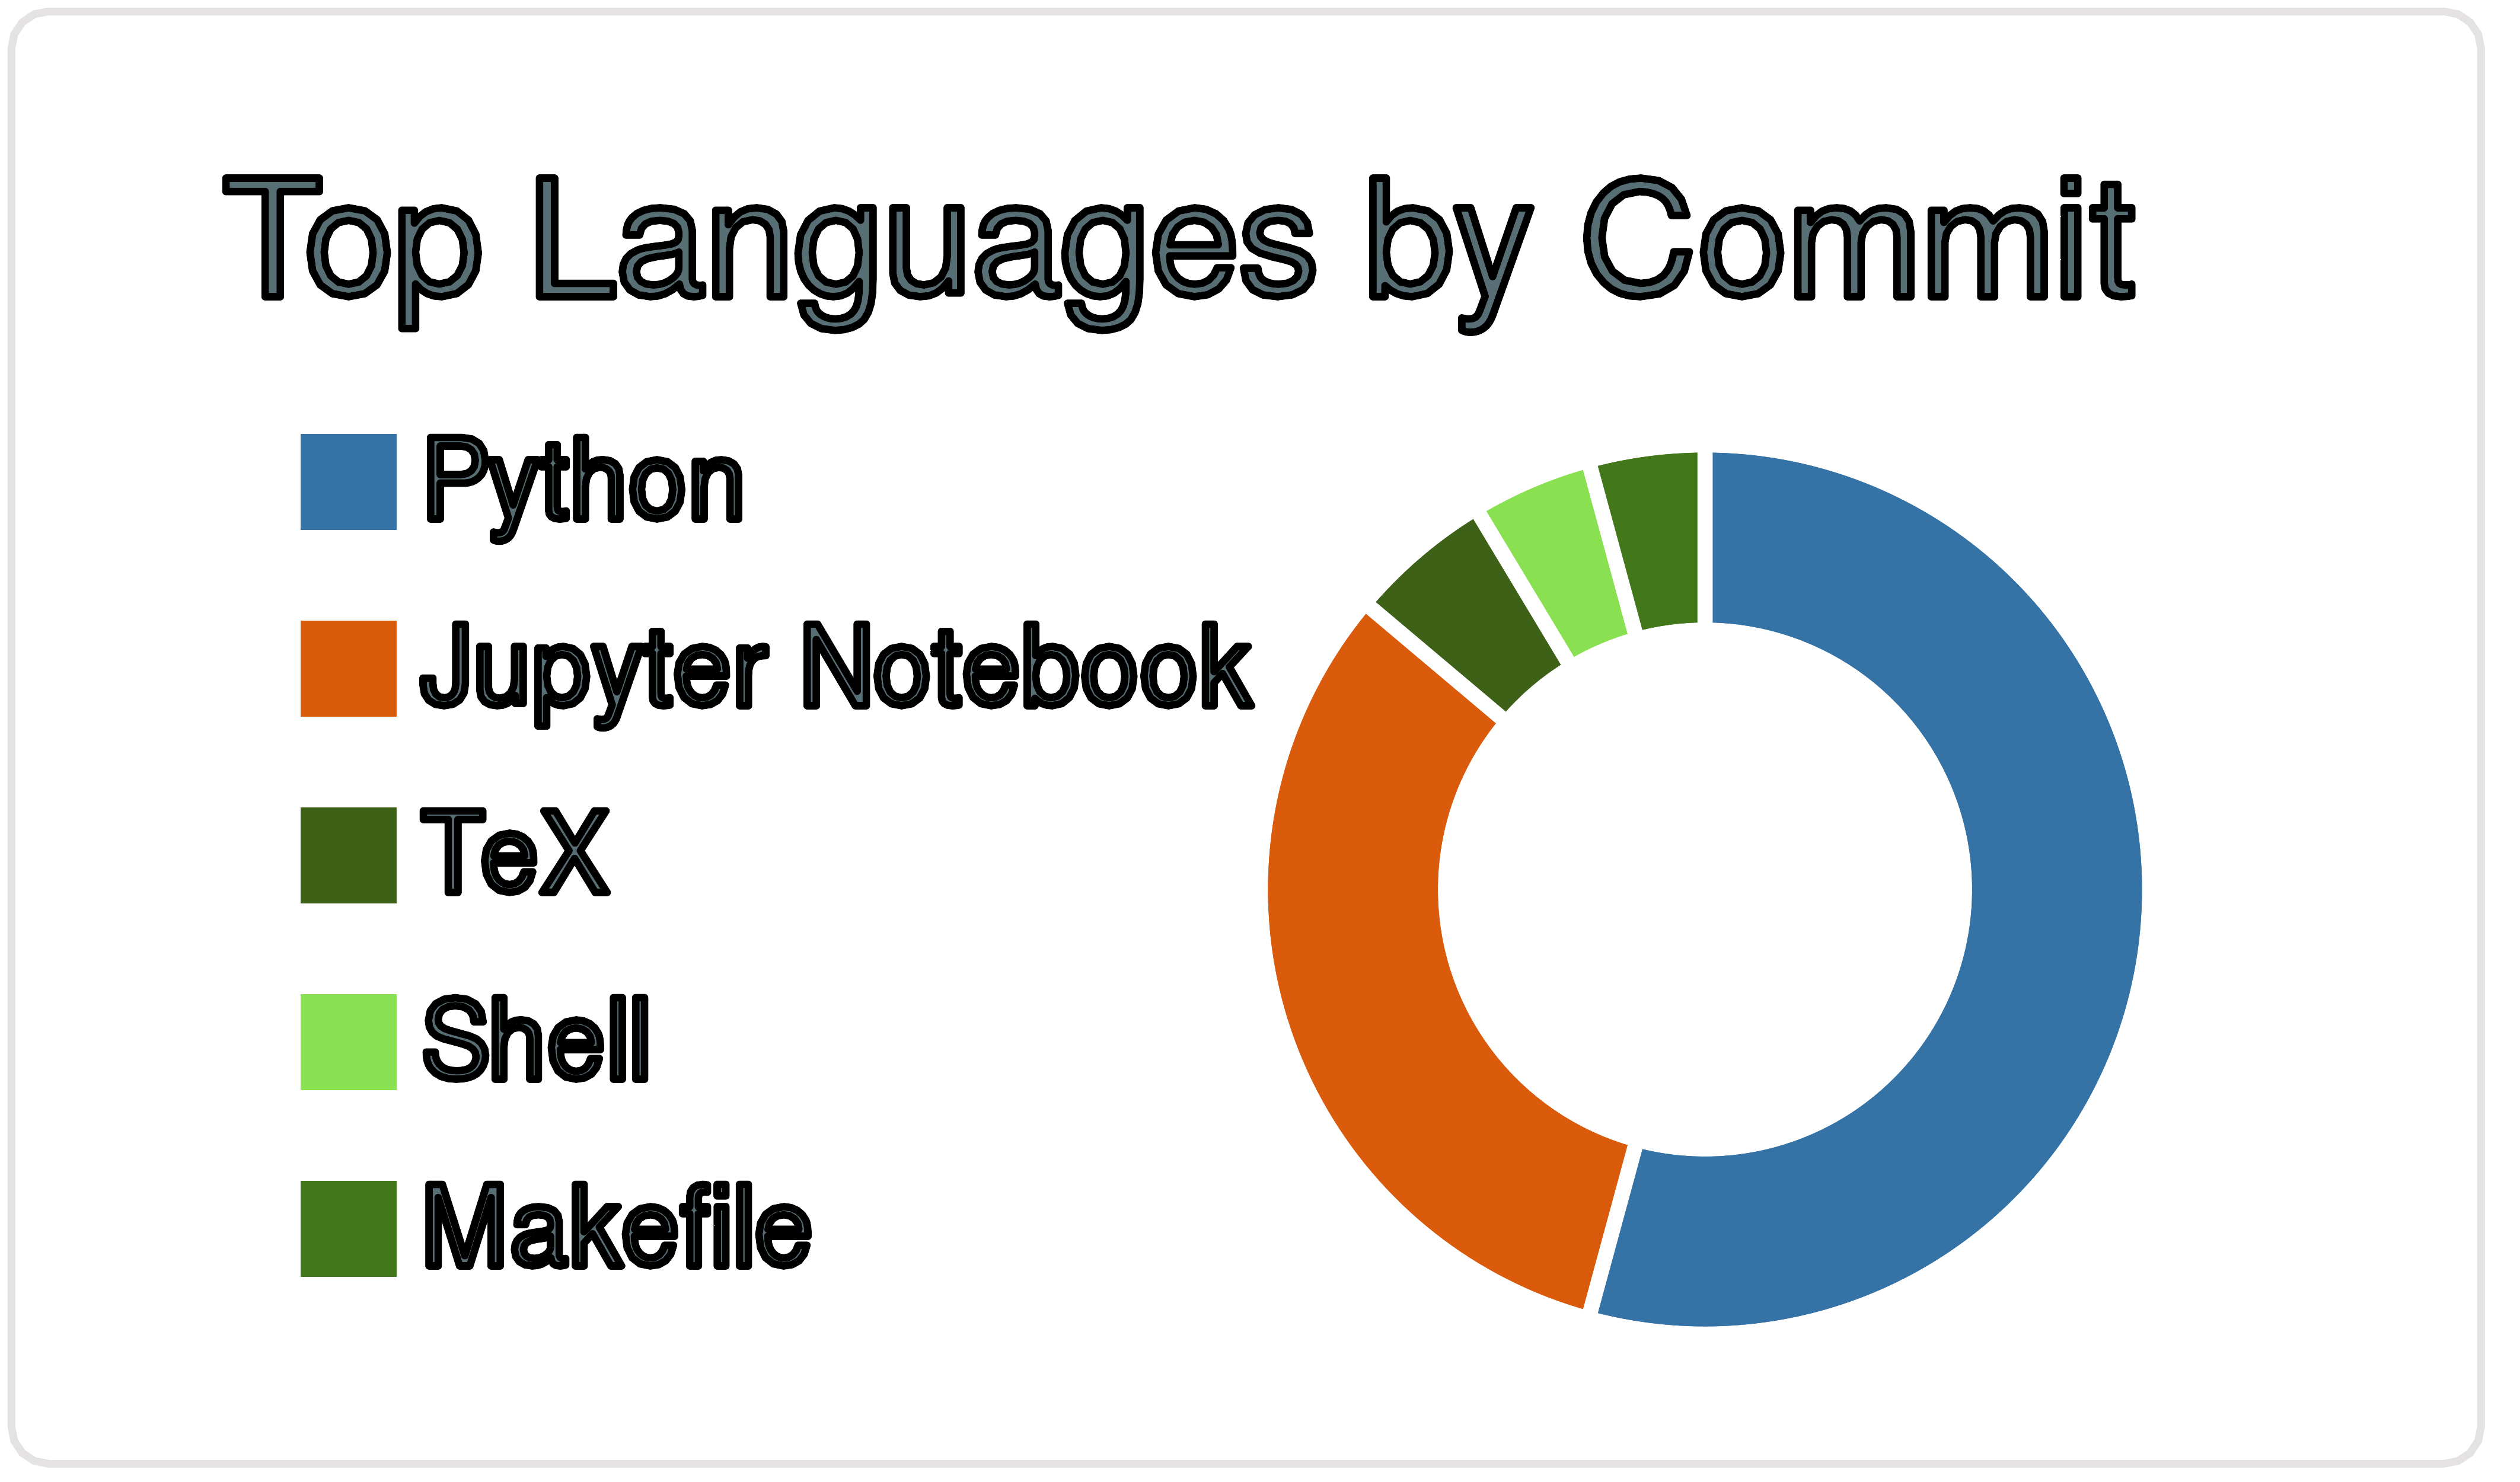
\includegraphics[width=0.50\linewidth]{2-most-commit-language.png}
\end{textblock*}
\note{
私のTwitterとGithubのアカウントは\href{https://twitter.com/tkoyama010}{@tkoyama010}です。

}
\note{
このプレゼンテーションを気に入っていただけたら、ぜひフォローしてください。
}
\end{frame}

\begin{frame}[fragile]
\begin{textblock*}{350pt}(50pt, 10pt)
\begin{block}{Hello World!}
\lstinputlisting[caption=Hello World!, label=hello_world_code, firstline=1, lastline=100]{hello_world.py}
\end{block}
\end{textblock*}
\end{frame}
\note{
コードリスト\ref{hello_world_code}では、\href{https://pypi.org/project/pyvista/}{PyVista}の "Hello World!" を行っています。
\href{https://pypi.org/project/pyvista/}{PyVista} スクリプトの基本ステップについて説明します。
まず、 \href{https://pypi.org/project/pyvista/}{PyVista} をインポートします。
次に \href{https://dev.pyvista.org/getting-started/what-is-a-mesh.html}{mesh} を生成して、それを
add meshメソッドを使用してPlotterオブジェクトに追加します。
}

\begin{frame}[fragile]
\begin{textblock*}{350pt}(50pt, 10pt)
\begin{block}{Hello World!}
\end{block}
\end{textblock*}
\begin{textblock*}{350pt}(50pt, 50pt)
\begin{block}{}
\begin{figure}
\includegraphics[width=1.0\linewidth]{hello_world.png}
\caption{Hello World!\label{HelloWorldFigure}}
\end{figure}
\note{
最後に、showメソッドを使って、PyVistaのレンダリングビュー(図 \ref{HelloWorldFigure})を確認します。
}
\end{block}
\end{textblock*}
\end{frame}

\begin{frame}[fragile]
\begin{textblock*}{350pt}(50pt, 10pt)
\begin{block}{Create tube from line}
\lstinputlisting[caption=Create tube, label=CreateTube, firstline=15, lastline=15]{tube.py}
\begin{figure}
\includegraphics[width=1.0\linewidth]{tube.png}
\caption{Line and tube\label{LineTubeFigure}}
\end{figure}
\end{block}
\end{textblock*}
\end{frame}
\note{
Tube関数を使用して、線の点から管のようなメッシュをカスタマイズすることもできます。
}

\begin{frame}[fragile]
\begin{textblock*}{200pt}(50pt, 10pt)
\begin{block}{Create PolyData}
\lstinputlisting[caption=Create PolyData, label=CreatePolyDataCode, firstline=12, lastline=29]{create-poly.py}
\end{block}
\end{textblock*}
\begin{textblock*}{350pt}(180pt, 50pt)
\begin{figure}
\includegraphics[width=0.5\linewidth]{create-poly.png}
\caption{Create PolyData \label{CreatePolyData}}
\end{figure}
\end{textblock*}
\end{frame}
\note{
メッシュをさらにカスタマイズする場合は、頂点と面のNumPy配列からPolyData (Triangulated Surface) オブジェクトを作成することもできます。
PolyDataオブジェクトは、numpy配列からすばやく作成できます。
頂点配列にはメッシュ内のポイントの位置が含まれ、面配列には各面のポイント数と、その面を構成する頂点のインデックスが含まれます。
}

\begin{frame}[fragile]
\begin{textblock*}{350pt}(50pt, 10pt)
\begin{block}{Load and plot from a files}
\lstinputlisting[caption=Load meshs from the many supported file formats, label=ReadFileCode, firstline=5, lastline=8]{read_file.py}
\begin{figure}
\includegraphics[width=0.6\linewidth]{read_file.png}
\caption{Meshs from the many supported file formats\label{ReadFileFigure}}
\end{figure}
\end{block}
\end{textblock*}
\end{frame}
\note{
ファイルからメッシュをロードすることもできます。
\href{https://dev.pyvista.org/getting-started/what-is-a-mesh.html}{mesh} のロードは簡単です。
データがサポートされている多くのファイルフォーマットのいずれかである場合、
単に \href{https://dev.pyvista.org/utilities/utilities.html}{pyvista.read()} を使用して空間的に参照されたデータセットを
\href{https://pypi.org/project/pyvista/}{PyVista} \href{https://dev.pyvista.org/getting-started/what-is-a-mesh.html}{mesh} オブジェクトにロードします
(コードリスト\ref{ReadFileCode}、図\ref{ReadFileFigure})。
}

\begin{frame}[fragile]
\begin{textblock*}{350pt}(50pt, 10pt)
\begin{block}{Load and plot from a files}
\lstinputlisting[caption=Save meshs to the many supported file formats, label=SaveFileCode, firstline=26, lastline=29]{read_file.py}
\begin{figure}
\includegraphics[width=0.6\linewidth]{read_file.png}
\caption{Meshs from the many supported file formats\label{ReadFileFigure}}
\end{figure}
\end{block}
\end{textblock*}
\end{frame}
\note{
また、任意の \href{https://pypi.org/project/pyvista/}{PyVista} メッシュを \href{https://pypi.org/project/meshio/}{meshio} でサポートされている任意のファイルフォーマットにエクスポートできることにも注意してください。
meshioを使って \href{https://pypi.org/project/pyvista/}{PyVista} のメッシュを保存するには、 \href{https://dev.pyvista.org/utilities/utilities.html}{pyvista.save\_meshio()} を使います(コードリスト \ref{SaveFileCode} )。
}

\begin{frame}[fragile]
\begin{textblock*}{350pt}(50pt, 10pt)
\begin{block}{Thresholding Filter}
\lstinputlisting[caption=Create tube, label=ThresholdingFilterCode, firstline=36, lastline=36]{using-filters.py}
\begin{figure}
\includegraphics[width=1.0\linewidth]{using-filters1.png}
\caption{Thresholding\label{ThresholdingFilterFigure}}
\end{figure}
\end{block}
\end{textblock*}
\end{frame}
\note{
このスライドではしきい値設定やクリッピングなどの一般的なフィルタを使用してみます。
PyVistaでラップされたデータオブジェクトには、オブジェクト上で直接すぐに使用できる一連の共通フィルタが用意されています。
これらのフィルタを使用するには、データ・オブジェクトで直接選択したメソッドを呼び出します。
これで、新しいしきい値オブジェクトに入力データセットのしきい値バージョンがあります。
フィルタの実行方法を変更するために使用できるキーワード引数の詳細については、ヘルプを使用するか、
IPython環境でshift+tabを使用して、PyVistaオブジェクトに適用されているフィルタのdocstringを出力してください。
}

\begin{frame}[fragile]
\begin{textblock*}{200pt}(20pt, 10pt)
\begin{block}{Using Common Filters}
\lstinputlisting[caption=Using Common Filters, label=using_common_filters, firstline=68, lastline=87]{using-filters.py}
\end{block}
\end{textblock*}
\begin{textblock*}{200pt}(250pt, 0pt)
\begin{figure}
\includegraphics[width=1.0\linewidth]{using-filters2.png}
\caption{Using Common Filters\label{UsingCommonFiltersFigure}}
\end{figure}
\end{textblock*}
\end{frame}
\note{
他のフィルターはどうですか?
いくつかのフィルタ結果を収集して比較します。
これはしきい値、コンター、スライス、グリフの図です。
}


\begin{frame}[fragile]
\begin{textblock*}{200pt}(20pt, 10pt)
\begin{block}{Filter Pipeline}
\lstinputlisting[caption=Filter Pipeline, label=using_common_filters, firstline=106, lastline=111]{using-filters.py}
\end{block}
\end{textblock*}
\begin{textblock*}{200pt}(250pt, 50pt)
\begin{figure}
\includegraphics[width=1.0\linewidth]{using-filters3.png}
\caption{Filter Pipeline\label{FilterPipelineFigure}}
\end{figure}
\end{textblock*}
\end{frame}
\note{
PyVistaでは、チェーンを介してフィルタリングパイプラインを模倣することができます。
各フィルタを最後のフィルタにアタッチします。
この例では、複数のフィルタが連結されています。
まず、すべてのNaN値を消去する空のしきい値フィルタです。
次に、高度フィルタを使用して、高さに対応するスカラー値を生成します。
さらに、クリップフィルタを使用してデータセットを半分にカットします。
最後に、slice\_orthogonalフィルタを使用して、各軸平面に沿って3つのスライスを作成します。
フィルタされたデータを表示するには、plotメソッド (result.plot () ) を呼び出すか、レンダリングシーンを作成します。
}

\begin{frame}[fragile]
\begin{textblock*}{350pt}(50pt, 10pt)
\begin{block}{Shrink mesh}
\lstinputlisting[caption=Shrink Mesh, label=ShrinkFilterCode, firstline=5, lastline=6]{shrunk_mesh.py}
\begin{figure}
\includegraphics[width=1.0\linewidth]{shrink.png}
\caption{Shrink filter\label{ShrinkFilterFigure}}
\end{figure}
\end{block}
\end{textblock*}
\end{frame}
\note{
メッシュの確認に便利なフィルターもあります。
コードリスト \ref{ShrinkFilterCode} では、shrinkメソッドを使ってメッシュの各面を縮小しています(図 \ref{ShrinkFilterFigure})。
}

\begin{frame}[fragile]
\begin{textblock*}{350pt}(50pt, 10pt)
\begin{block}{Clip with Plane}
\lstinputlisting[caption=Clip with Plane, label=ClipWithPlaneCode, firstline=20, lastline=21]{clipping.py}
\begin{figure}
\includegraphics[width=1.0\linewidth]{clipping1.png}
\caption{Clip with Plane\label{ClipWithPlane}}
\end{figure}
\end{block}
\end{textblock*}
\end{frame}
\note{
pyvistaを使用して、pyvista.DataSetFilters.clip() フィルタを使うことで、ユーザ定義平面によりデータセットをクリップすることもできます。
}

\begin{frame}[fragile]
\begin{textblock*}{350pt}(50pt, 10pt)
\begin{block}{Clip with Bounds}
\lstinputlisting[caption=Clip with Bounds, label=ClipWithBoundsCode, firstline=39, lastline=42]{clipping.py}
\begin{figure}
\includegraphics[width=1.0\linewidth]{clipping2.png}
\caption{Clip with Bounds\label{ClipWithBounds}}
\end{figure}
\end{block}
\end{textblock*}
\end{frame}
\note{
pyvistaを使用して、XYZ境界のセットによってデータセットをクリップします。
DataSetFilters.clip\_box () フィルタです。
}

\begin{frame}[fragile]
\begin{textblock*}{350pt}(50pt, 10pt)
\begin{block}{Rotation about the x axis}
\note{
もちろん、軸を中心にメッシュを回転させることもできます。
メッシュを軸周りに回転させてみましょう。
このモデルでは、x軸は左から右へ、y軸は下から上へ、z軸は画面から垂直になっています。
カメラの位置は2つの画像で同じです。
このメッシュをx軸を中心に60度ごとに回転させてプロットできます。
もちろん、他の軸についてもプロットできます。
}
\end{block}
\lstinputlisting[caption=X-Axis Rotation, firstline=66, lastline=69]{rotate.py}
\begin{figure}
\includegraphics[width=1.0\linewidth]{rotate_x.png}
\caption{X-Axis Rotation}
\end{figure}
\end{textblock*}
\end{frame}

\begin{frame}[fragile]
\begin{textblock*}{350pt}(50pt, 10pt)
\begin{block}{Rotation about the y axis}
\note{
メッシュを60度ごとにY軸を中心に回転させてプロットします。
プロッターに軸アクターを追加し、軸の原点を回転点に設定しています。
}
\end{block}
\lstinputlisting[caption=Y-Axis Rotation, firstline=66, lastline=69]{rotate.py}
\begin{figure}
\includegraphics[width=1.0\linewidth]{rotate_y.png}
\caption{Y-Axis Rotation}
\end{figure}
\end{textblock*}
\end{frame}

\begin{frame}[fragile]
\begin{textblock*}{350pt}(50pt, 10pt)
\begin{block}{Rotation about the z axis}
\note{
メッシュを60度ごとにz軸を中心に回転させてプロットします。
プロッターに軸アクターを追加し、軸の原点を回転点に設定しています。
}
\end{block}
\lstinputlisting[caption=Z-Axis Rotation, firstline=66, lastline=69]{rotate.py}
\begin{figure}
\includegraphics[width=1.0\linewidth]{rotate_z.png}
\caption{Z-Axis Rotation}
\end{figure}
\end{textblock*}
\end{frame}

\begin{frame}[fragile]
\begin{textblock*}{350pt}(50pt, 10pt)
\begin{block}{Rotation about a custom vector}
\note{
メッシュを60度ごとのカスタムベクトルで回転させてプロットします。
プロッターに軸アクターを追加し、軸の原点を回転点に設定しています。
}
\end{block}
\lstinputlisting[caption=Custom Rotation, firstline=66, lastline=69]{rotate.py}
\begin{figure}
\includegraphics[width=1.0\linewidth]{rotate_custom.png}
\caption{Custom Rotation}
\end{figure}
\end{textblock*}
\end{frame}

\begin{frame}[fragile]
\begin{textblock*}{350pt}(50pt, 10pt)
\begin{block}{General filters to any data type}
\lstinputlisting[caption=Extrude Rotate, label=ExtrudeRotateCode, firstline=7, lastline=9]{extrude_rotate.py}
\begin{figure}
\includegraphics[width=1.0\linewidth]{extrude_rotate.png}
\caption{Extrude Rotation\label{ExtrudeRotateFigure}}
\end{figure}
\note{
コードリスト \ref{ExtrudeRotateCode} では、押出し回転メソッドを使って直線から "skirt" を
作成しています (図\ref{ExtrudeRotateFigure}) 。
}
\end{block}
\end{textblock*}
\end{frame}

\begin{frame}[fragile]
\begin{textblock*}{350pt}(50pt, 10pt)
\begin{block}{Extracting and Contouring}
\lstinputlisting[caption=Extracted by scalar, label=WarpScalarCode, firstline=9, lastline=9]{contour.py}
\begin{figure}
\includegraphics[width=0.5\linewidth]{contour.png}
\caption{Contouring\label{WarpScalarFigure}}
\end{figure}
\note{
Attributeとは、メッシュのノードまたはセル上に存在するデータ値のことです。
\href{https://pypi.org/project/pyvista/}{PyVista} では、ポイントデータとセルデータの両方を扱い、メッシュのすべてのノードまたはすべてのセルに存在する属性の配列を保持するデータ辞書に簡単にアクセスできるようにしています。
\href{https://dev.pyvista.org/core/filters.html}{warp\_by\_scalar()} メソッドでメッシュからスカラーフィールドを抽出することができます(コードリスト \ref{WarpScalarCode} 、図 \ref{WarpScalarFigure} )。
}
\end{block}
\end{textblock*}
\end{frame}

\begin{frame}[fragile]
\begin{textblock*}{350pt}(50pt, 10pt)
\begin{block}{Plot data over circular arc}
\lstinputlisting[caption=Plotting over circular arc, label=PlotOverCircularArcCode, firstline=10, lastline=18]{kitchen.py}
\end{block}
\end{textblock*}
\begin{textblock*}{300pt}(0pt, 110pt)
\begin{block}{}
\note{
\href{https://dev.pyvista.org/core/filters.html}{plot\_over\_circular\_arc\_normal}
を使用して、データセットを通る円弧上のデータセットの値をプロットすることができます
(コードリスト\ref{PlotOverCircularArcCode}、図\ref{CircularArcToPlotFigure}および\ref{PlotOverCircularArcFigure})。
}
\begin{figure}
\includegraphics[width=0.5\linewidth]{kitchen.png}
\caption{Circular arc to plot \label{CircularArcToPlotFigure}}
\end{figure}
\end{block}
\end{textblock*}
\begin{textblock*}{350pt}(150pt, 130pt)
\begin{figure}
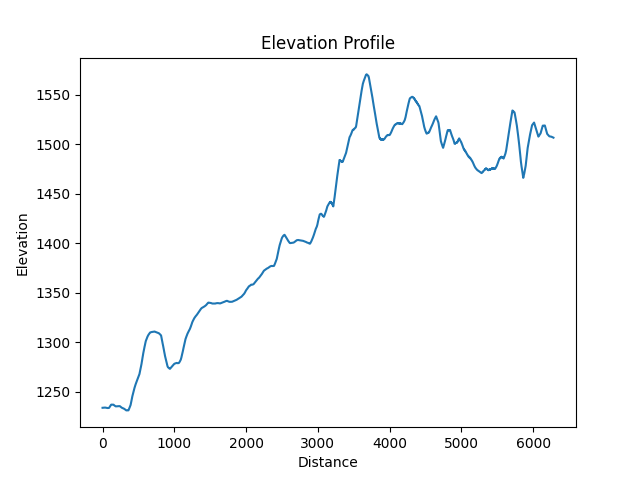
\includegraphics[width=0.3\linewidth]{elevation.png}
\caption{Plot over line \label{PlotOverCircularArcFigure}}
\end{figure}
\end{textblock*}
\end{frame}

\begin{frame}[fragile]
\begin{textblock*}{350pt}(50pt, 10pt)
\begin{block}{Extracting and Contouring}
\lstinputlisting[caption=Extracted by vector, label=WarpVectorCode, firstline=44, lastline=44]{contour.py}
\begin{figure}
\includegraphics[width=1.0\linewidth]{warped_vector.png}
\caption{Warped sphere by vector\label{WarpVectorFigure}}
\end{figure}
\end{block}
\end{textblock*}
\end{frame}
\note{
また、 \href{https://dev.pyvista.org/core/filters.html}{warp\_by\_vector()} メソッドで抽出されたベクターファイルを持つことができます(コードリスト \ref{WarpVectorCode} 、図 \ref{WarpVectorFigure} )。
\href{https://dev.pyvista.org/plotting/plotting.html}{add\_mesh () }メソッドは、スカラー値をプロットするときにMatplotlib、Colorcet、cmocean、またはカスタムカラーマップを使用できます (図\ref{WarpVectorFigure}) 。
}

\begin{frame}[fragile]
\begin{textblock*}{350pt}(50pt, 10pt)
\begin{block}{Silhouette Highlight}
\lstinputlisting[caption=Silhouette Highlight, label=SilhouetteHighlight, firstline=22, lastline=28]{silhouette.py}
\begin{figure}
\includegraphics[width=1.0\linewidth]{silhouette1.png}
\caption{Silhouette Highlight\label{WarpVectorFigure}}
\end{figure}
\end{block}
\end{textblock*}
\end{frame}
\note{
ポリゴンメッシュのエッジのサブセットを抽出し、add\_meshメソッドを使用してメッシュのアウトラインシルエットを生成できます。
シルエット引数で設定することができます。
}

\begin{frame}[fragile]
\begin{textblock*}{350pt}(50pt, 10pt)
\begin{block}{Camera class}
\begin{figure}
\includegraphics[width=0.75\linewidth]{frustum_of_camera.png}
\caption{Frustum of camera \label{CameraFrustumFigure}}
\end{figure}
\note{
\href{https://dev.pyvista.org/core/camera.html}{Camera}クラスは、3Dレンダリング用の仮想カメラです。
視点や焦点の位置や方向を決めるメソッドを提供します。
また、焦点を移動するための便利なメソッドも提供されています。
より複雑なメソッドでは、ビューアップベクター、クリッピングプレーン、カメラパースペクティブなど、コンピュータグラフィックスモデルを操作することができます(図 \ref{CameraFrustumFigure})。
}
\lstinputlisting[caption=Add Camera to Plotter, label=camera_view, firstline=7, lastline=13]{camera_view.py}
\end{block}
\end{textblock*}
\end{frame}

\begin{frame}[fragile]
\begin{textblock*}{350pt}(50pt, 10pt)
\begin{block}{Camera class}
\lstinputlisting[caption=Create camera frustum, label=CameraFrustumCode, firstline=8, lastline=13]{frustum_of_camera.py}
\begin{figure}
\includegraphics[width=0.75\linewidth]{camera_view.png}
\caption{Camera view}
\end{figure}
\note{
コードリスト\ref{CameraFrustumCode}ではカメラと視錐台を作成しています。
次に、視錐台内部のシーンを作成して、\href{https://dev.pyvista.org/plotting/plotting.html}{Plotter}オブジェクトに\href{https://dev.pyvista.org/core/camera.html}{Camera}オブジェクトを追加します
(コードリスト\ref{CameraFrustumCode}、図\ref{CameraFrustumFigure})。
}
\end{block}
\end{textblock*}
\end{frame}

\begin{frame}[fragile]
\begin{textblock*}{150pt}(50pt, 10pt)
\begin{block}{Controlling Camera Rotation}
\lstinputlisting[caption=Controlling Camera Rotation, label=CameraRotationCode, firstline=29, lastline=29]{camera_view.py}
\lstinputlisting[firstline=34, lastline=34]{camera_view.py}
\lstinputlisting[firstline=39, lastline=39]{camera_view.py}
\end{block}
\end{textblock*}
\begin{textblock*}{350pt}(150pt, 50pt)
\begin{figure}
\includegraphics[width=0.5\linewidth]{camera_rotation.png}
\caption{Controlling Camera Rotation \label{CameraRotationFigure}}
\end{figure}
\note{
さらに、pyvistaの\href{https://dev.pyvista.org/core/camera.html}{Camera.position}
プロパティを使用してカメラ位置を設定することにより、カメラ位置を直接制御することもできます。
カメラの
\href{https://dev.pyvista.org/core/camera.html}{pyvista.Camera.roll},
\href{https://dev.pyvista.org/core/camera.html}{pyvista.Camera.elevation},
および\href{https://dev.pyvista.org/core/camera.html}{pyvista.Camera.azimuth}
を直接制御することもできます。
(コードリスト\ref{CameraRotationCode}、図\ref{CameraRotationFigure})
}
\end{textblock*}
\end{frame}

\begin{frame}[fragile]
\begin{textblock*}{350pt}(50pt, 10pt)
\begin{block}{Light Types}
\lstinputlisting[caption=Headlight, label=Headlight, firstline=32, lastline=36]{light_types.py}
\begin{figure}
\includegraphics[width=1.0\linewidth]{light_types1.png}
\caption{Headlight\label{Headlight}}
\end{figure}
\end{block}
\end{textblock*}
\end{frame}
\note{
光の状態を設定することもできます。
光源には3つのタイプがあります。
1つ目はヘッドライトです。
軸は常にカメラのビューと一致します。
ヘッドライトの場合、positionプロパティとfocal\_pointプロパティは意味がありません。
カメラをどこに移動しても、ライトは常に視点から放射されます。
}

\begin{frame}[fragile]
\begin{textblock*}{350pt}(50pt, 10pt)
\begin{block}{Light Types}
\lstinputlisting[caption=Cameralight, label=Cameralight, firstline=54, lastline=56]{light_types.py}
\begin{figure}
\includegraphics[width=1.0\linewidth]{light_types2.png}
\caption{Cameralight\label{Cameralight}}
\end{figure}
\end{block}
\end{textblock*}
\end{frame}
\note{
2つ目はカメラライトです。カメラライトは、カメラに対してローカルな座標系で位置とfocal\_pointプロパティを定義します。
シーンの座標系の座標には、それぞれworld\_positionおよびworld\_focal\_point読み取り専用プロパティからアクセスできます。
座標に使用されるローカル座標系の詳細については、pyvistaLight.set\_camera\_light()のドキュメントを参照してください。
}

\begin{frame}[fragile]
\begin{textblock*}{350pt}(50pt, 10pt)
\begin{block}{Light Types}
\lstinputlisting[caption=Scenelight, label=Scenelight, firstline=69, lastline=71]{light_types.py}
\begin{figure}
\includegraphics[width=1.0\linewidth]{light_types3.png}
\caption{Scenelight\label{Scenelight}}
\end{figure}
\end{block}
\end{textblock*}
\end{frame}
\note{
3つ目はシーンライトです。
シーンライトはシーンにアタッチされ、その位置と焦点はグローバル座標として解釈されます。
}

\begin{frame}[fragile]
\begin{textblock*}{350pt}(50pt, 10pt)
\begin{block}{Types of Shading}
\lstinputlisting[caption=Types of Shading, label=TypesofShading, firstline=19, lastline=23]{shading.py}
\begin{figure}
\includegraphics[width=1.0\linewidth]{shading.png}
\caption{Types of Shading\label{TypesOfShading}}
\end{figure}
\end{block}
\end{textblock*}
\end{frame}
\note{
ライトを使用する場合は、シェーディングも重要です。
PyVistaでは、フラットシェーディングとスムーズシェーディングの2種類のシェーディングがサポートされています。
これは、既定のフラットシェーディングとスムーズシェーディングを使用したプロットです。
}

\begin{frame}[fragile]
\begin{textblock*}{350pt}(50pt, 10pt)
\begin{block}{Eye Dome Lighting}
\lstinputlisting[caption=Eye Dome Lighting, label=EyeDomeLighting, firstline=40, lastline=40]{edl.py}
\begin{figure}
\includegraphics[width=1.0\linewidth]{edl1.png}
\caption{Statue\label{Statue}}
\end{figure}
\end{block}
\end{textblock*}
\end{frame}
\note{
アイドームライティング (EDL) は、科学的可視化イメージの奥行き知覚を改善するために設計された、非フォトリアリスティックなイメージベースのシェーディングテクニックです。
アイドームライティングは、クリエイティブ・コモンズのネフェルティティ女王の像のような非常に洗練されたメッシュを描画するときに、奥行きの知覚を劇的に改善します。
ここでは、EDLシェーディングと通常のシェーディングを並べて比較します。
}

\begin{frame}[fragile]
\begin{textblock*}{350pt}(50pt, 10pt)
\begin{block}{Eye Dome Lighting}
\lstinputlisting[caption=Eye Dome Lighting, label=EyeDomeLighting, firstline=40, lastline=40]{edl.py}
\begin{figure}
\includegraphics[width=1.0\linewidth]{edl2.png}
\caption{Point Cloud\label{PointCloud}}
\end{figure}
\end{block}
\end{textblock*}
\end{frame}
\note{
単純な点群を印刷する場合、奥行きを認識するのが難しいことがあります
たとえば、このライダー点群を考えてみましょう。
次に、この点群をそのまま描画します。
}

\begin{frame}[fragile]
\begin{textblock*}{350pt}(50pt, 10pt)
\begin{block}{Applying Textures}
\lstinputlisting[caption=Applying Textures, label=EyeDomeLighting, firstline=27, lastline=29]{texture.py}
\begin{figure}
\includegraphics[width=1.0\linewidth]{texture1.png}
\caption{Applying Textures\label{ApplyingTextures}}
\end{figure}
\end{block}
\end{textblock*}
\end{frame}
\note{
また、イメージをテクスチャとして投影したメッシュをプロットすることもできます。
テクスチャマッピングは、PyVistaを使用して簡単に実装できます。
ジオメトリックオブジェクトの多くにはテクスチャ座標があらかじめロードされているため、サーフェスをすばやく作成してイメージを表示するには、次の操作を実行します。
}

\begin{frame}[fragile]
\begin{textblock*}{350pt}(50pt, 10pt)
\begin{block}{Physically Based Rendering (PBR)}
\lstinputlisting[caption=Physically Based Rendering (PBR), label=PBR, firstline=35, lastline=37]{pbr.py}
\begin{figure}
\includegraphics[width=1.0\linewidth]{pbr1.png}
\caption{Physically Based Rendering (PBR) Textures\label{PBRFigure}}
\end{figure}
\end{block}
\end{textblock*}
\end{frame}
\note{
VTK 9はPhysically Based Rendering (PBR) を導入し、その機能をPyVistaで公開しました。
PBRは、pyvistaでのみサポートされています。PolyDataであり、add\_meshのpbrキーワード引数を介してトリガできます。
さらにコントロールするには、metallic引数とroughness引数も使用します。
ここでは、彫像の高品質のメッシュをメタリックであるかのようにレンダリングして、この機能を紹介します。
メッシュを 「リネン」 のベースカラーでレンダリングして、金属のような仕上げにします。
}

\begin{frame}[fragile]
\begin{textblock*}{350pt}(50pt, 10pt)
\begin{block}{Physically Based Rendering (PBR)}
\lstinputlisting[caption=Physically Based Rendering (PBR), label=PBR, firstline=35, lastline=37]{pbr.py}
\begin{figure}
\includegraphics[width=1.0\linewidth]{pbr2.png}
\caption{Physically Based Rendering (PBR) Textures\label{PBRFigure}}
\end{figure}
\end{block}
\end{textblock*}
\end{frame}
\note{
この図は金属と粗さのパラメータの変化を示しています。
左から右に向かって金属の属性が増加し、下から上に向かって粗さが増加するようにプロットしています。
}

\begin{frame}[fragile]
\begin{textblock*}{350pt}(50pt, 10pt)
\begin{block}{Box Widget}
\lstinputlisting[caption=Box Widget, label=BoxWidgetList, firstline=30, lastline=32]{box-widget.py}
\end{block}
\begin{figure}
\movie[width=5cm,height=5cm]{}{box-clip.gif}
\end{figure}
\end{textblock*}
\end{frame}
\note{
PyVistaには、クリッピング、スライス、しきい値などのフィルタを制御するためにレンダリングシーンに追加できるウィジェットがいくつかあります。
ボックスウィジェットは、ピビスタで有効または無効にできます。WidgetHelper.add\_box\_widget () およびpyvista。それぞれWidgetHelper.clear\_box\_widgets () メソッド。
ボックスウィジェットを有効にするときは、カスタムコールバック関数を提供する必要があります。
そうしないと、ボックスが表示されて何も実行されません。
コールバック関数を使用すると、ウィジェットを利用してクリッピングやクロップなどのタスクを実行できます。
}

\begin{frame}[fragile]
\begin{textblock*}{800pt}(50pt, 10pt)
\begin{block}{Conclusion}
\note{
matplotlibのようにPythonicな方法で3Dデータを可視化したいなら、このスライドはあなたのためのものです。
このスライドは、 \href{https://pypi.org/project/pyvista/}{PyVista} の紹介です。これは
}
\begin{itemize}
\item "VTK for humans"\: a high-level API to the Visualization Toolkit (VTK)
\note[item]{
"VTK for humans"\: a high-level API to the Visualization Toolkit (VTK).
}
\item 3D plotting made simple and built for large/complex data geometries
\note[item]{
大規模/複雑なデータ形状に対応した、シンプルな3Dプロッティング機能があります
}
\item mesh data structures and filtering methods for spatial datasets
\note[item]{
メッシュデータ構造と空間データのフィルタリング方法があります。
}
\end{itemize}
\end{block}
\end{textblock*}
\begin{textblock*}{800pt}(50pt, 150pt)
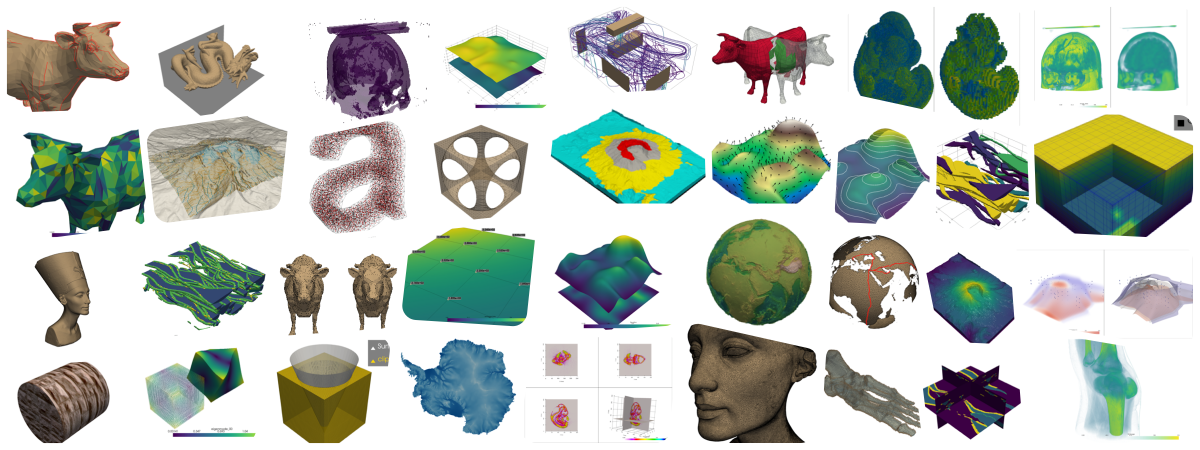
\includegraphics[width=0.50\linewidth]{pyvista_banner_small.png}
\end{textblock*}
\end{frame}

\begin{frame}[fragile]
\begin{textblock*}{800pt}(50pt, 10pt)
\begin{block}{Conclusion}
We introduce the PyVista's
\begin{itemize}
\item Pythonic interface to VTK’s Python bindings
\item Filtering/plotting tools built for interactivity
\item Direct access to common VTK filters
\item Intuitive plotting routines with matplotlib similar syntax
\end{itemize}
\end{block}
\end{textblock*}
\begin{textblock*}{800pt}(50pt, 150pt)
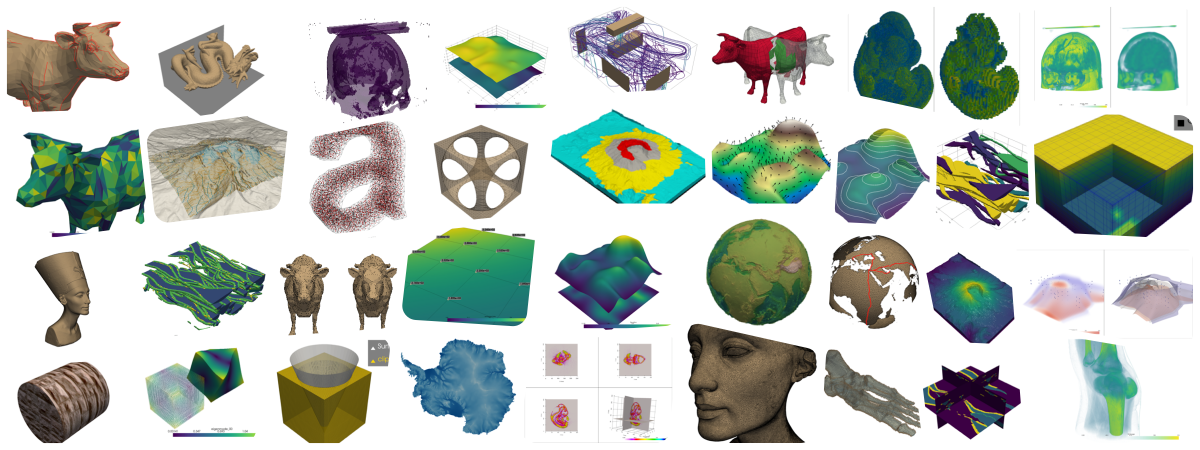
\includegraphics[width=0.50\linewidth]{pyvista_banner_small.png}
\end{textblock*}
\end{frame}
\note{
このプレゼンテーションでは、PyVistaが異なるVTKメッシュタイプをどのようにラップするか、そして強力な3Dプロットとメッシュ解析ツールをどのように活用するかについて詳しく説明しました。
このAPIのハイライトは以下の通りです。

VTKのPythonバインディングへのPythonicインターフェース

インタラクティブ性を重視したフィルタリング/プロットツール(ウィジェットを参照)

一般的なVTKフィルタへの直接アクセス (フィルタを参照)

matplotlibに似た構文を持つ直感的なプロットルーチン (プロットを参照)

}



\begin{frame}[fragile]
\begin{textblock*}{350pt}(50pt, 10pt)
\begin{block}{Acknowlegment}
I would like to thank \href{https://github.com/orgs/pyvista/teams/developers}{PyVista developer team} for developing useful library.
\end{block}
\begin{block}{References}
C. Bane Sullivan and Alexander Kaszynski, (2019). PyVista: 3D plotting and mesh analysis through a streamlined interface for the Visualization Toolkit (VTK). Journal of Open Source Software, 4(37), 1450, \url{https://doi.org/10.21105/joss.01450}
\end{block}
\begin{block}{Contact Information}
If you want to know and discuss pyvista more, join \href{http://github.com/pyvista/pyvista/discussions}{GitHub Discussion}.
\end{block}
\doclicenseThis
\end{textblock*}
\end{frame}
\note{
役に立つライブラリを開発してくれたPyVista開発チームに感謝します。
このプレゼンテーションは"PyVista: 3D plotting and mesh analysis through a streamlined interface for the Visualization Toolkit (VTK). Journal of Open Source Software."を参考文献としました。
pyvistaについてもっと知りたいなら、\href{http://github.com/pyvista/pyvista/discussions}{GitHub Discussion}に参加してください。
}

\end{document}

